\chapter{Architektura systemu}

System został napisany jako aplikacja webowa z~użyciem wzorca architektonicznego Model-Widok-Kontroler (ang. Model-View-Controller, MVC). Wzorzec ten zakłada podział aplikacji na 3 części:

\begin{enumerate}
\item model (ang. model) - który odpowiada za dane i~logikę biznesową;
\item widok (ang. view) - który odpowiada na interfejs, za pomocą którego użytkownik komunikuje się z~aplikacją;
\item kontroler (ang. controller) - który odpowiada za interakcję z~użytkownikiem, przyjmuje od niego dane wejściowe (przekazane za pomocą widoku), przetwarza informacje a~następnie aktualizuje model i/lub widok;
\end{enumerate}

\begin{figure}[!h]
\centering
    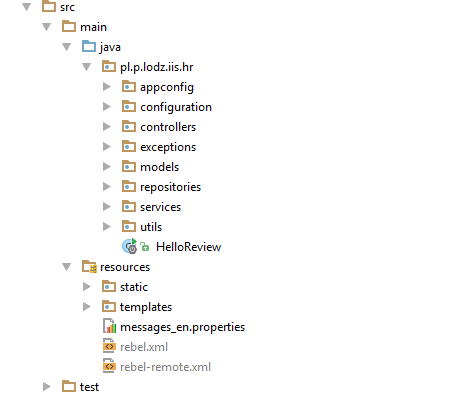
\includegraphics[width=360px]{0_1struktura}
    \caption{Architektura systemu - struktura plików}
    \label{obr01}
\end{figure}

\clearpage
Rysunek \ref{obr01} przedstawia strukturę plików w~projekcie. System składa kolejno z~takich pakietów jak:

\begin{itemize}

\item appconfig - zawiera klasy odpowiedzialne za odczyt z~pliku konfiguracji systemu; 

\item configuration - zawiera klasy odpowiedzialne za skonfigurowanie systemu, to znaczy skonfigurowanie bazowej platformy Spring Boot, połączenie z~nią używanych zależności (innych technologii), konfigurację serwera http;

\item controllers - klasy wchodzące w~skład warstwy kontroler. Odbierają żądania http, przekazują komunikaty do modelu, i~renderują odpowiedni widok zawierający odpowiedź;

\item exceptions - wydzielona część warstwy kontroler. Zawiera deklaracje klas odpowiedzialnych za obsługę sytuacji wyjątkowych;

\item models - część warstwy model. Zawiera encje - klasy odpowiadające za składowanie danych;

\item repositories - część warstwy model. Warstwa pośrednia pomiędzy sterownikiem dostępu do bazy danych, a~encjami. Zawiera, zgodnie ze wzorem repozytorium (ang. repository pattern), klasy umożliwiające operacje typu CRUD (utwórz, odczytaj, zaktualizuj, usuń; ang: create, read, update, delete), oraz operacje selekcji warunkowych w~systemie bazodanowym;

\item servives - część warstwy model. Zawiera usługi operujące na encjach, w~praktyce ten pakiet zawiera logikę biznesową;

\item utils - dodatkowe klasy narzędziowe, nie związane bezpośrednio z~aplikacją, lecz użyteczne przy jej tworzeniu;

\item resources/static - część warstwy view. Zawiera wszystkie pliki statyczne, które nie zależą od kontekstu wykonania, takie jak: obrazki, pliki skryptów JavaScript, arkusze styli CSS;

\item resources/templates - część warstwy view. Zawiera szablony generowane dynamicznie, zależne od kontekstu, i~danych przekazanych do nich poprzez kontroler.

\end{itemize}

\clearpage
Zastosowana struktura pakietów trochę rozdrabnia ogólny podział, który jest zdefiniowany przez wzorzec MVC. Wynika to z~naturalnej tendencji do separacji klas, które łączy wspólna cecha oraz chęci tworzenia systemu warstwowego, o~prostej strukturze zależności. Szkic założonej architektury zawiera rysunek \ref{obr02}.

\begin{figure}[!h]
\centering
    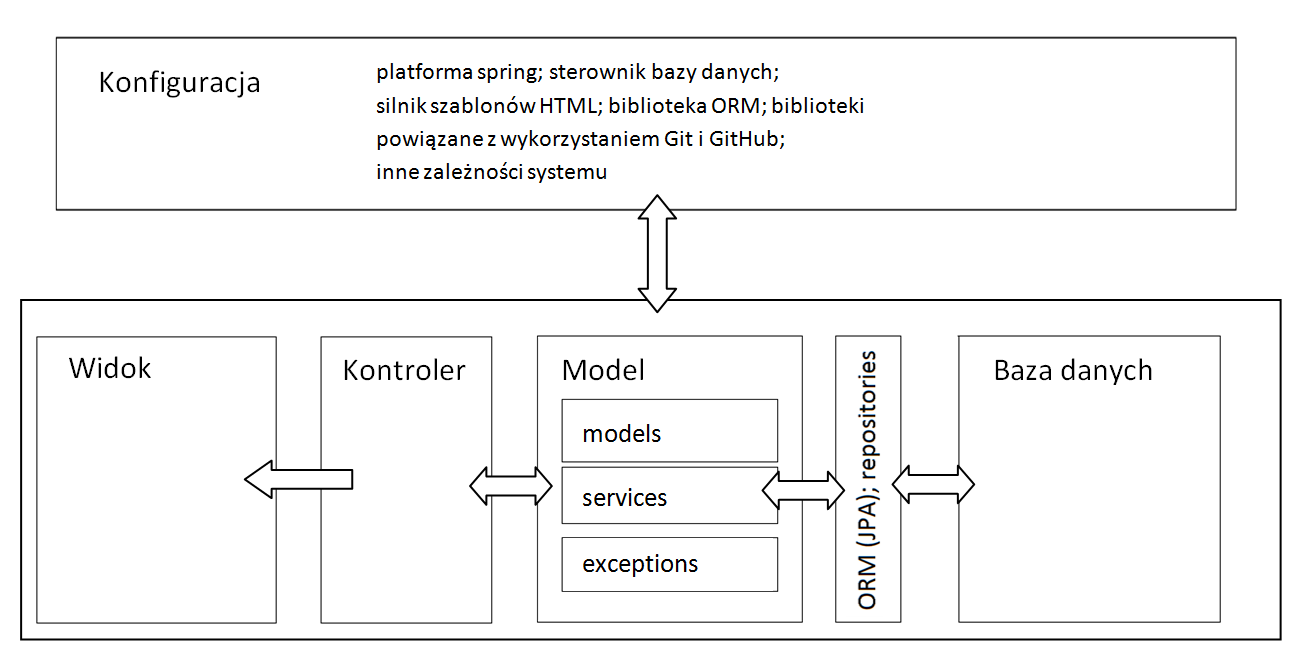
\includegraphics[width=\textwidth]{0_2architektura}
    \caption{Architektura systemu - zależność pakietów}
    \label{obr02}
\end{figure}

% ex: set tabstop=4 shiftwidth=4 softtabstop=4 noexpandtab fileformat=unix filetype=tex spelllang=pl,en spell: